\documentclass[10pt]{article}
\usepackage[utf8]{inputenc}
\usepackage[english]{babel}
\usepackage[T1]{fontenc}
\usepackage{amsmath}
\usepackage{amsfonts}
\usepackage{amssymb}
\usepackage{makeidx}
\usepackage{graphicx}
\usepackage{lmodern}
\usepackage{subfigure}
\usepackage{kpfonts}
\usepackage{caption}
\usepackage{tabto}

\author{262719}
\title{\begin{huge}
Linear Models
\end{huge}\\Data Analysis Project}
\date{}
\begin{document}
\maketitle
 
\tableofcontents
\newpage

\section{Introduction}
\quad The goal of this report is to discuss the factors affecting the concentration of prostate specific antigen (PSA). For our analysis we will first describe the methods that we will use and then construct a Gaussian linear model for the data. We will then interpret the results and discuss the strengths and weaknesses of this approach. Finally we will propose improvements for further investigations.

\section{The Data}
\quad We will base our analysis on the dataset published in Journal of Urology 141(5), 1989, pp 1076-1083. The dataset contains 8 variables and 97 observations and was collected on men before they underwent radical prostatectomy, a surgical procedure during which the prostate gland is removed. The data comes from a study that examined the correlation between PSA and several clinical measures. 

\begin{table}[ht]
\centering
\caption{Variables in prostate dataset} \label{datadescript}
\begin{tabular}{cl}
  \hline
 Column & Description \\ 
  \hline
1 & Log of cancer volume (in milliliters) \\
2 & Log of prostate weight (in grams)  \\
3 & Age of patient (in years)  \\
4 & Log of the amount of benign prostatic hyperplasia (cm${^2}$) \\
5 & Seminal vesical invasion (0 = No, 1 = Yes)  \\
6 & Log of the capsular penetration (in cm)  \\
7 & Gleason score (2-10)  \\
8 & Percentage of Gleason score that are 4 or 5 (0 to 100) \\ 
9 & Log of prostate specific antigen (in ng/ml) \\
   \hline
\end{tabular}
\end{table}


\section{Methodology and Outline}
\quad  We will first fit a Gaussian linear model to the data [1] with the PSA as the response while incorporating all possible covariates and then check with diagnostic plots that the 4 assumptions inherent to this model hold in this context: namely linearity, homoskedasticity, and the independence and gaussianess of the error terms [2]. We will also look for leverage points [3] and outliers as well [4] as try to assess the level of collinearity of the data. Once this done we will fit all possible models corresponding to all different combinations of covariates and select the model which has the lowest Bayesian Information Criterion (BIC) [5]. We will also build a model with backward selection [6]. In the next step we will add interactions between the covariates selected and then compare all models produced. We will then select the final model by comparing several metrics: their Akaike Information Criterion (AIC) [7], their BIC, the Variance Inflation Factors of their respective parameters (VIF) [8] and their adjusted R squared [9]. Finally we will interpret our results and criticize them.

\section{Analysis}
\quad Let's start with a matrix scatterplot of the data to see if a Gaussian linear model is appropriate for the data and if transformations of the covariates are necessary. 

\begin{figure}[htb]
\begin{center}
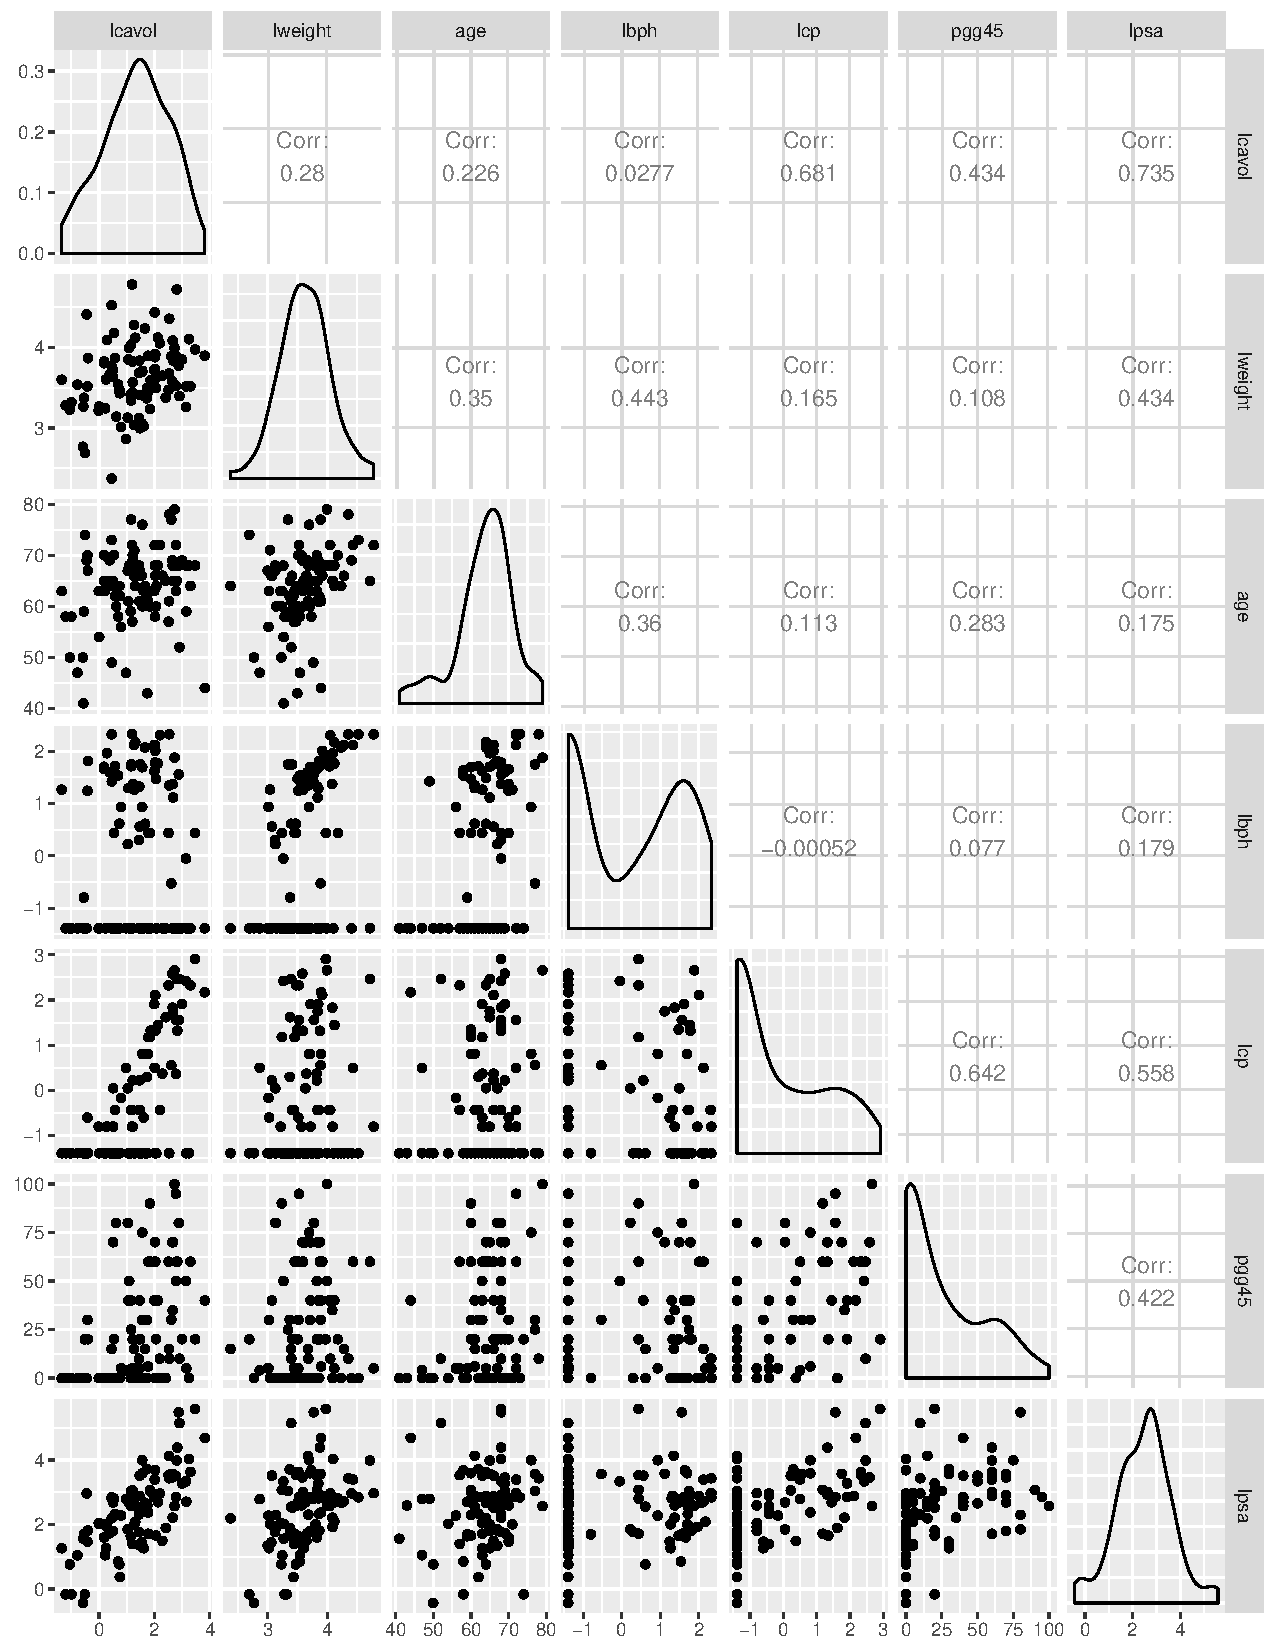
\includegraphics[height=4in,width=5in]{matrixscatterplot.pdf}
\caption{Matrix scatterplot of all covariates}
\end{center}
\end{figure}

As we can see on Figure 1 such a model seems appropriate in this case since the PSA varies linearly with respect to the covariates. We can also conclude than no further transformations of the variables is necessary. One can also see that some covariates seems heavily correlated with each other which could pose problems later on. Next we see that we need to treat svi and gleason as indicator variables. Further data exploration shows that there is exactly one observation with a Gleason score of 8 which we will remove from the data since it will act as a leverage point for the whole model.

\begin{figure}[htb]
\begin{center}
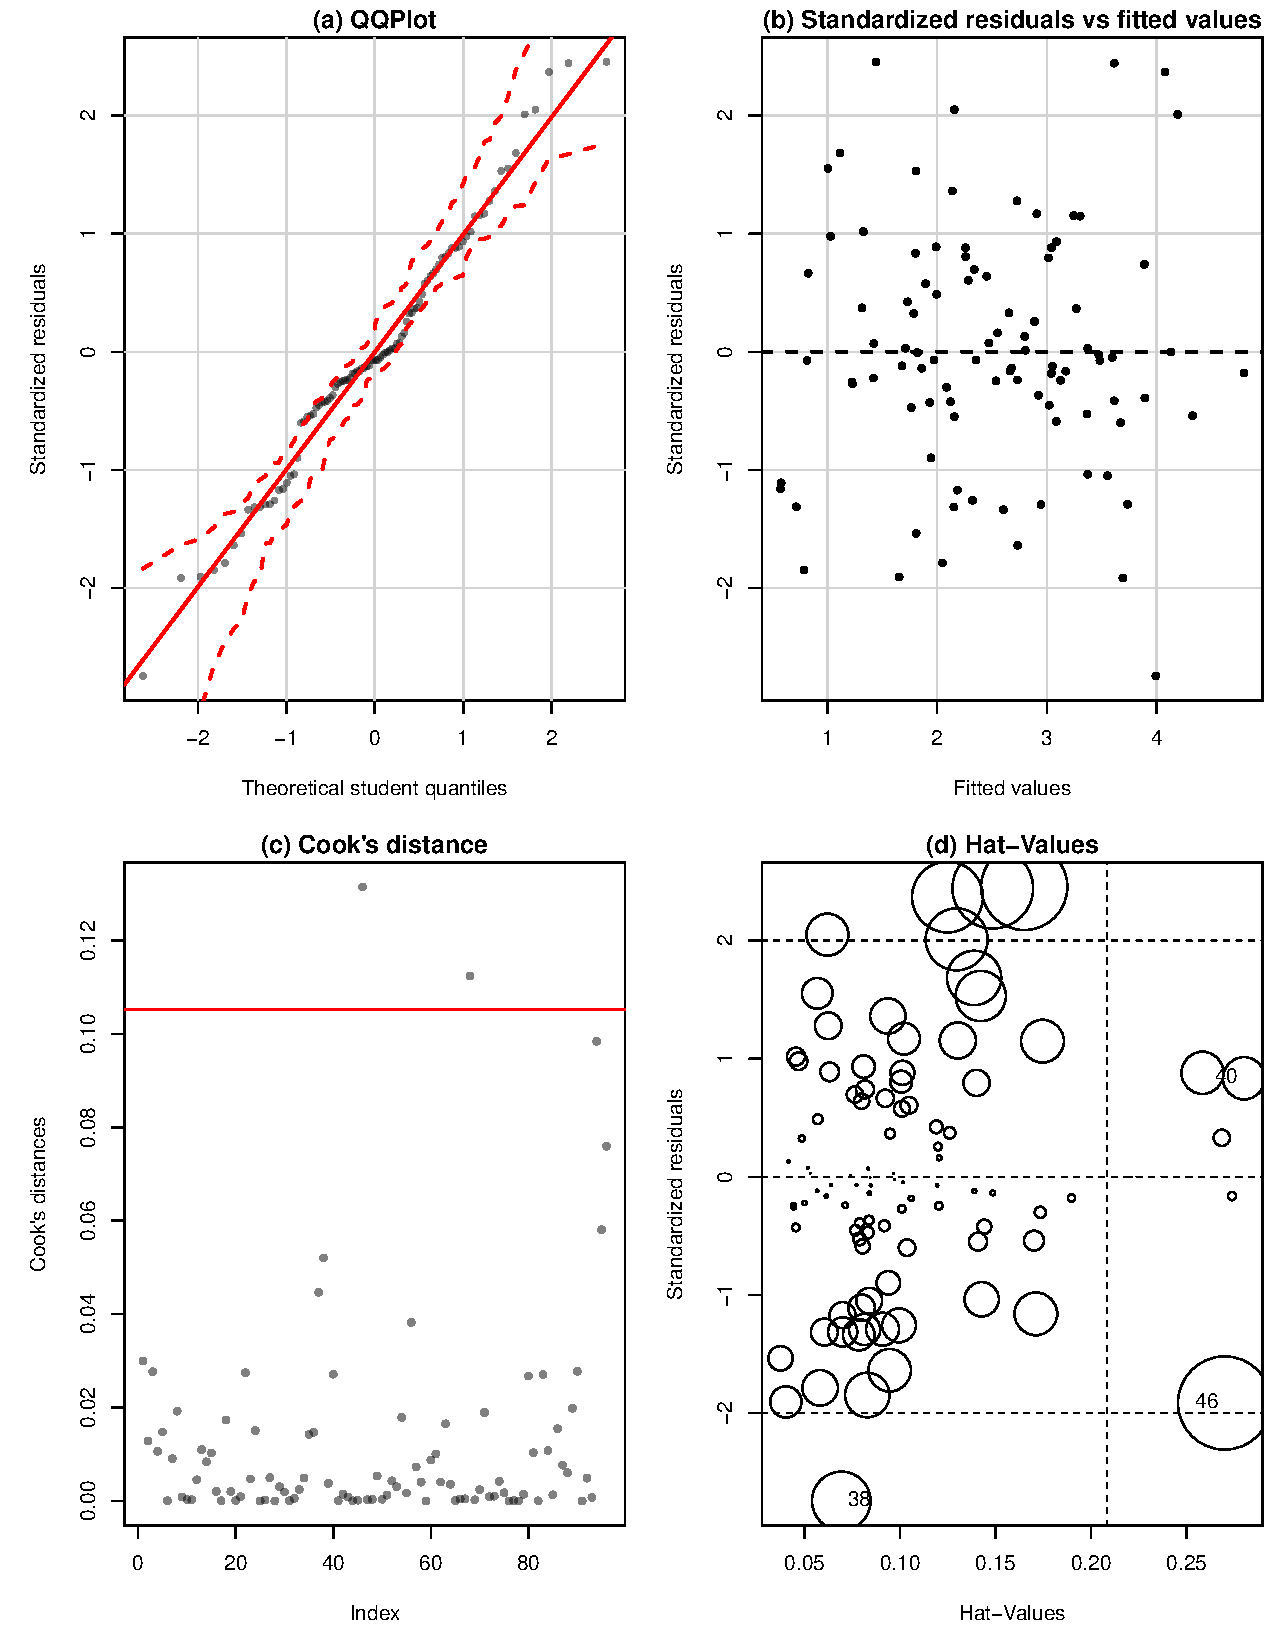
\includegraphics[height=4in,width=5in]{diagnostics_full_model.pdf}
\caption{Diagnostic plots}
\end{center}
\end{figure}

We now fit the full model (Model 1) as described in the outline and look at the diagnostic plots produced. By looking at covariates vs residuals plots we realise that the hypothesis of linearity of the response with respect to the explanatories holds since no pattern emerges from the plots. In Figure 2 (b) homoskedasticity  is respected since we observe no trumpet or curved pattern. Furthermore we can see in Figure 2 (a) that the hypothesis of normality of the errors seems respected since the quantiles of our standardized residuals correspond to a student distribution. Finally by look at Figure 2 (c) and (d) we can see that there are 3 observations that exert an abnormal influence on the plot: observations 39,41 and 47. By looking at their associated residuals we can conclude that 39 is an outlier (r = -2.74) and that 41 and 47 are leverage points. Finally we see see that the condition number of the matrix [10] is 883.33 which shows that indeed our data exhibits pathological multicollinearity. In this study we will only flag these two problems while still proposing ways to deal with them later in further investigations.

Next we try to build a better model by using both backward selection and by fitting all possible models and then selecting the one with the lowest BIC. Both methods result in the same model (Model 2) and only include the log cancer volume (lcavol), the log prostate weight (lweight) and the seminal vesicle invasion indicator (svi) as covariates. We will build two more model by adding interactions between lcavol and lweight (Model 3) and lcavol and svi (Model 4). We now compare the models produced.

\begin{table}[ht]
\centering
\caption{Comparison of models built} \label{criteriontable}
\begin{tabular}{rrrrr}
  \hline
 & Model 1 & Model 2 & Model 3 & Model 4 \\ 
  \hline
AIC & 214.64 & 212.87 & 211.76 & 214.8 \\ 
BIC & 242.85 & 225.69 & 227.15 & 230.18 \\ 
Adj R squared & 0.639 & 0.624 & 0.632 & 0.620 \\ 
  \hline
\end{tabular}
\end{table}

By looking at Table 1 we see that both Model 2 and Model 3 have minimal AIC/BIC and similar R squared values. But if we compare the VIFs of their parameters we see that those of Model 3 are substantially higher which means that this model will be hardly interpretable. Furthermore we will also select Model 2 since it is simpler than Model 3.

\section{Interpretation and Discussion}

\quad Let's now interpret our results. We first start by looking at a summary of the model selected:

\begin{table}[ht]
\centering
\caption{Summary model selected} \label{summary}
\begin{tabular}{rrrrr}
  \hline
 & Estimate & Std. Error & t value & Pr($>$$|$t$|$) \\ 
  \hline
(Intercept) & -0.776 & 0.626 & -1.240 & 0.218 \\ 
  lcavol & 0.527 & 0.075 & 6.998 & 0.000 \\ 
  lweight & 0.662 & 0.176 & 3.752 & 0.000 \\ 
  svi & 0.661 & 0.209 & 3.169 & 0.002 \\ 
   \hline
\end{tabular}
\end{table}

\begin{table}[ht]
\centering
\caption{VIF table} \label{summary}
\begin{tabular}{rrrrr}
  \hline
 & lcavol & lweight & svi \\ 
  \hline
VIF & 1.49 & 1.09 & 1.41 \\ 
   \hline
\end{tabular}
\end{table}

We see that all the variables chosen in the final model are deemed significant and that the VIFs of the parameters are at an acceptable level to try to interpret the model. The baseline level of PSA for a patient is 0.46 ng/ml according to this model. Furthermore we expect a 0.53\% increase in PSA levels when the cancer volume increases by 1\%, a 0.66\% increase when the weight of the prostate increases by 1\% and a 9.37\%  increase when in the presence of seminal vesicle invasion. We also didn't find any changes in PSA concentration that are due to interactions between the cancer volume and other variables.

The PSA is a protein produced by normal and malignant cells of the prostate, thus it is not surprising to see that the weight of the prostate aswell as the cancer volume will both have a positive impact on the levels of production of this protein. Indeed the heavier the prostate and the bigger the number of cancerous cells, the more they can produce PSA. The indication of a seminal vehicle invasion can also be a marker for a more aggressive form cancer, since it has spread to other areas, which means that the malignant cells are more biologically active and thus that they will produce more biological agents including PSA.

From this model we can see that there seems to be link between the level of PSA and the size and/or aggressiveness of a cancer, which means that PSA could potentially be used to detect prostate cancer: a higher concentration of PSA could indicate the presence of the sickness. However we can't be conclusive about this since our dataset contained only men known to have prostate cancer and we have no idea what are the concentration levels of this protein for healthy men or what are other non-pathological factors affecting its production.

As a final word it is important to note that our model is of little predictive value since it can't say anything about men with a Gleason score lower than 6 or equal to 8 and can only be applied for already sick men for which it certainly is not interesting to know the concentration of PSA.


\section{Conclusion}

\quad In conclusion we investigated the factors that affect the concentration of PSA and found that that the size of the prostate, the volume of the cancer and seminal vesicle invasion by cancerous cells all had a positive impact on it. However our dataset exhibited multicollinearity which we didn't address in this report but which could be tackled by applying Ridge Regression [11] in a further study. We also flagged several leverage/outlier points which ought to be looked at more closely, preferably by someone having more domain specific knowledge. Finally the potential use of PSA as a marker for prostate cancer should be investigated with new data including a control group of healthy men as it could lead to important applications in oncology.

\newpage

\section{Bibliography}

[1] Slides MATH-341 Linear Models class, slide 41 \newline
[2] Slides MATH-341 Linear Models class, slide 91 \newline
[3] Slides MATH-341 Linear Models class, slide 113 \newline
[4]Slides MATH-341 Linear Models class, slide 110 \newline
[5] Slides MATH-341 Linear Models class, slide 158 \newline
[6] Slides MATH-341 Linear Models class, slide 161 \newline
[7] Slides MATH-341 Linear Models class, slide 157 \newline
[8] Slides MATH-341 Linear Models class, slide 169 \newline
[9] Slides MATH-341 Linear Models class, slide 73 \newline
[10] Slides MATH-341 Linear Models class, slide 171 \newline
[11] Slides MATH-341 Linear Models class, slide 181 \newline

\end{document}